\subsection{Introducción}

En esta sección se implementó un filtro High-Pass, utilizando una aproximación \textbf{Cauer} e implementándola con celdas \textbf{Sedra}. El filtro diseñado cumple con la siguiente plantilla.
\begin{table}[H]
\centering
\begin{tabular}{|c|c|}
\hline
$f_s$      & 11.65 kHz          \\ \hline
$f_p$      & 23.3 kHz           \\ \hline
$A_p$      & 2 dB               \\ \hline
$A_s$      & 40 dB              \\ \hline
$|Z_{in}|$ & $\geq 50 \ k \Omega$ \\ \hline
\end{tabular}
\caption{Plantilla del filtro.}
\label{tab:plantilla}
\end{table}
\subsection{Aproximación de Cauer}
Se utilizó la aproximación elíptica de \textbf{Cauer}, además se propuso una plantilla mas restrictiva, con el fin de asegurar el cumplimiento de la original, siendo la plantilla final la presentada en la Tabla (\ref{tab:plantilla}).

Obteniendo la siguiente función transferencia, se expresa como producto de transferencias de segundo orden, teniendo los pares de polos con un Q de 0.84 la primer etapa y 4.17.
\begin{align}
	H(s)=\frac{ {s}^{2}+ 124088460.2 
 }{s^2+s\cdot 5466 + 519.84\cdot 10^6 } \cdot \frac{  {s}^{2}+
 23794591.32 }{s^2+s\cdot 48182 + 1.6\cdot 10^9 }
\label{eq:trans}
\end{align}
De esta forma, se presenta el diagrama de polos y ceros de dicha función:
\begin{figure}[H]
	\centering
	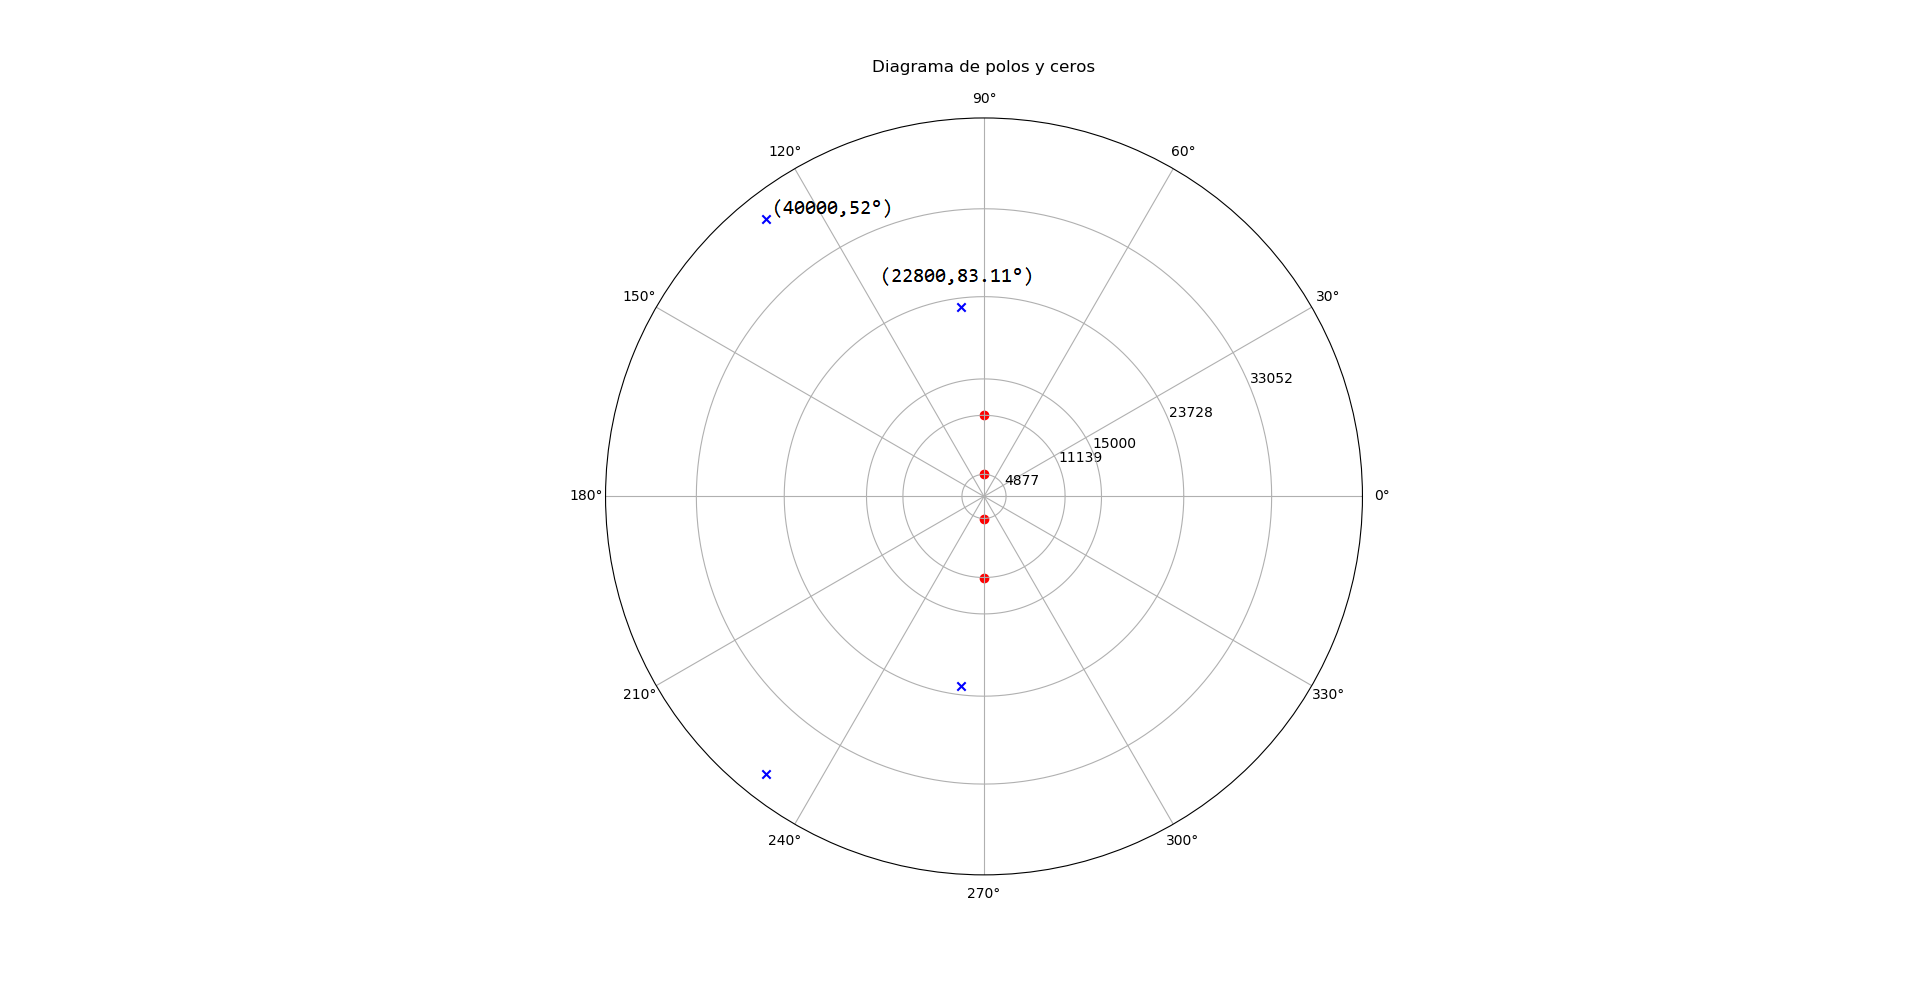
\includegraphics[width=\textwidth]{Imagenes-Ej3/DiagramaPolosYCeros.png}
	\label{fig:poleZeroDiag}
	\caption{Diagrama Polos y Ceros}
\end{figure}

Finalmente se graficó la respuesta en frecuencia tanto en fase como en módulo:
\begin{figure}[H]
	\centering
	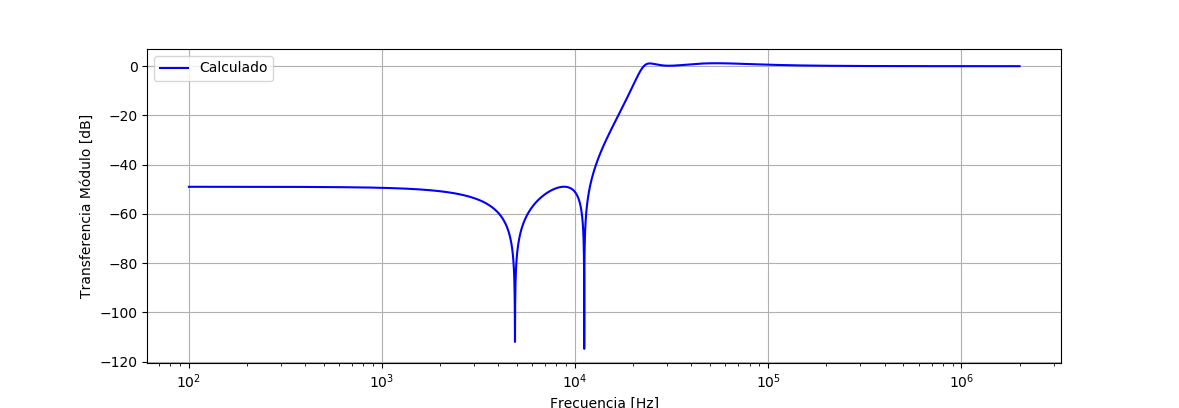
\includegraphics[width=\textwidth]{Imagenes-Ej3/BodeCalc.png}
	\caption{Diagrama de bode Módulo.}
	\label{fig:Bodecalc}
\end{figure}
\begin{figure}[H]
	\centering
	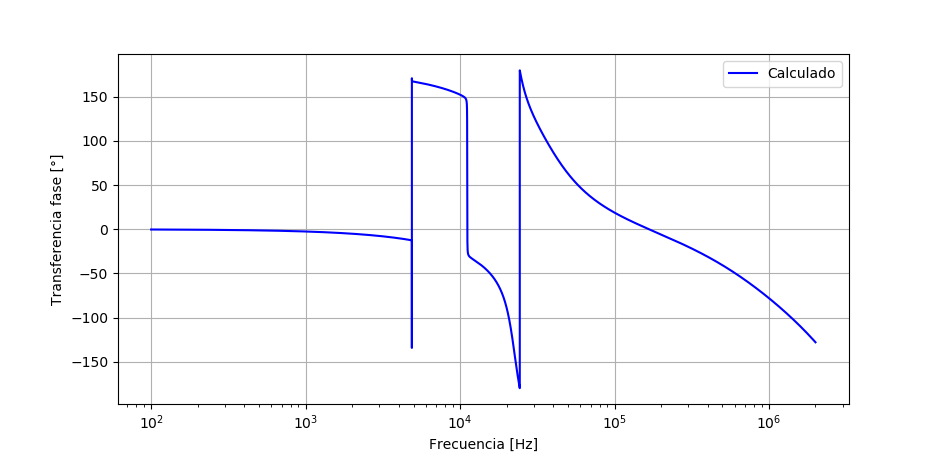
\includegraphics[width=\textwidth]{Imagenes-Ej3/BodeFaseCalc.png}
	\caption{Diagrama de bode Fase.}
	\label{fig:BodeCalcF}
\end{figure}
Se aclara que en la Figura ({fig:BodeCalcF}) la fase se encuentra acotada entre $-180 ^o$ y $180 ^o$. 

\subsubsection{Elecciones de diseño}
Se decidió armar etapas con celdas de segundo orden en cascada, dado a que el orden del filtro es de 4. Para la asociación de polos se tomó como criterio agrupar los polos por su cercanía, obteniendose así la siguiente forma.
\begin{figure}[H]
	\centering
	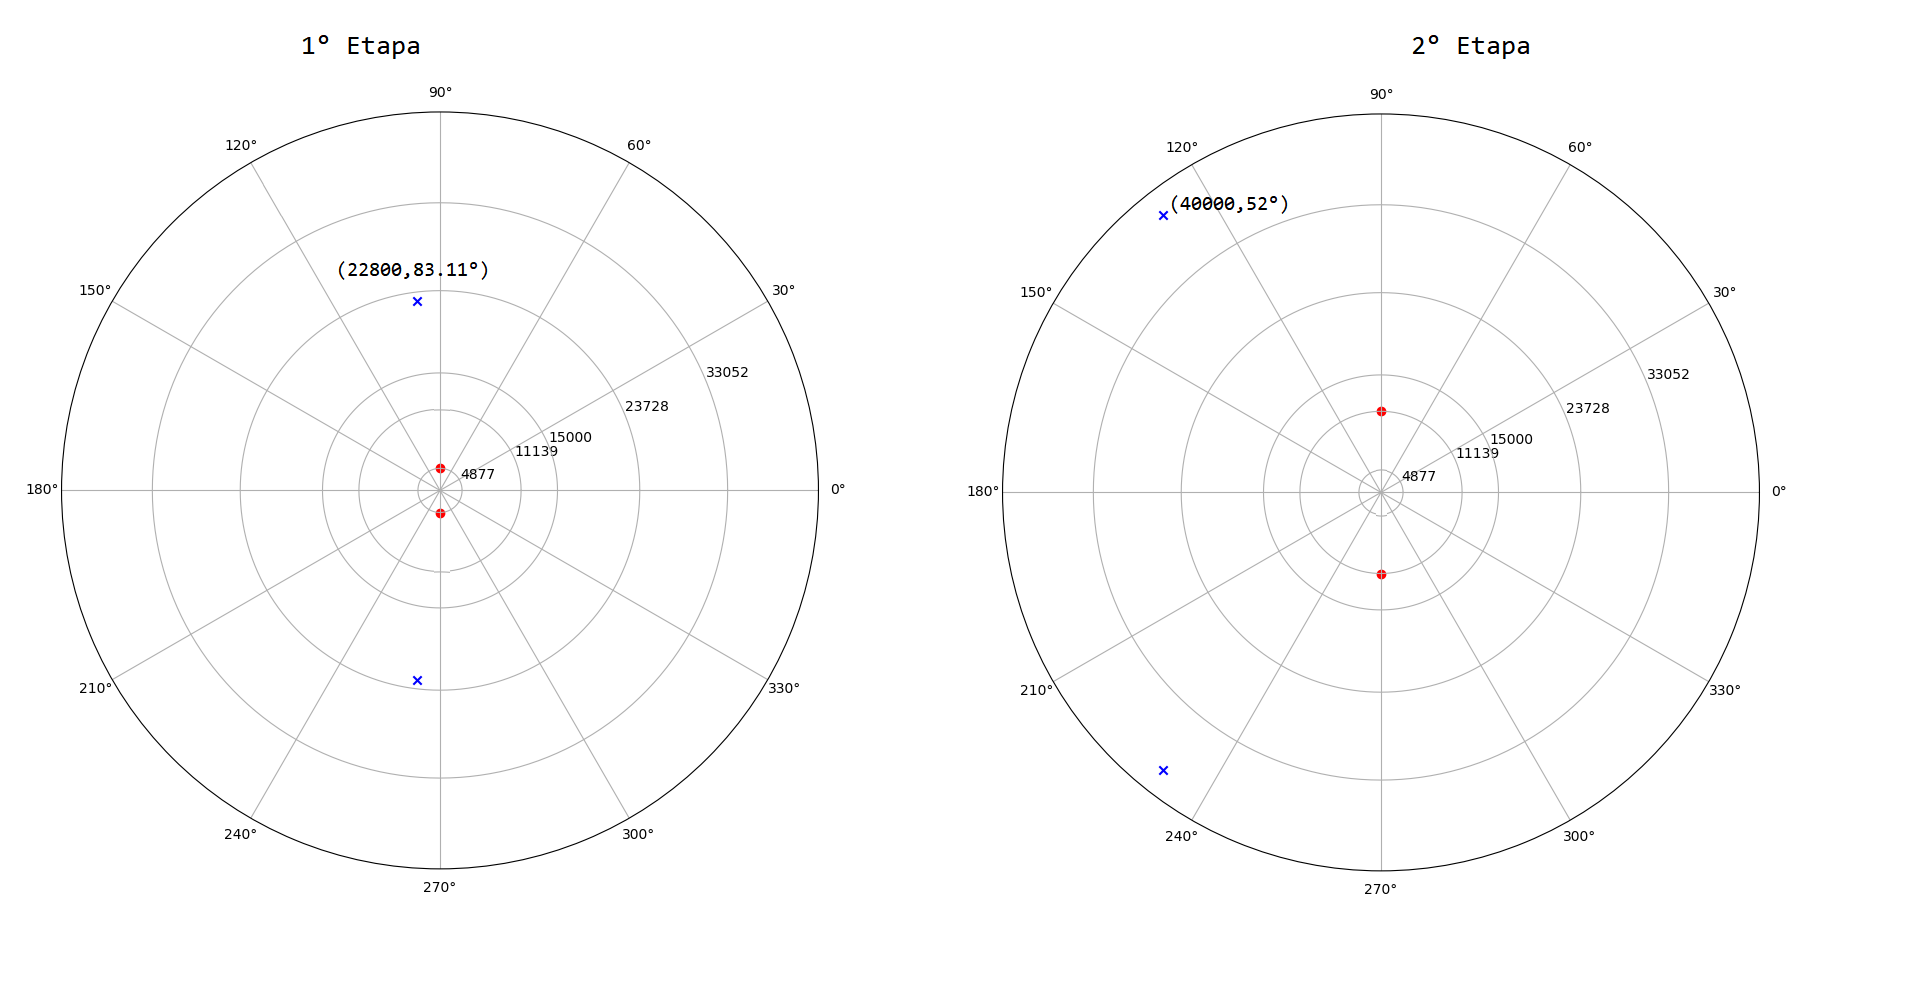
\includegraphics[width=\textwidth]{Imagenes-Ej3/UnionCeros.png}
	\caption{Diagrama Polos y Ceros para cada etapa}
	\label{fig:CeroPoleUnion}
\end{figure}

Una vez determinado esto, se optó por colocar la etapa de mayor Q al final.

\subsection{Celda Sedra-Ghorab-Martin}
La celda Sedra-Ghorab-Martin fue propuesta en el paper ``Optimum Configurations for Single Amplifiers Biquadratic Filters'', originalmente como una mejora de la celda Deliyannis. Es un diseño que permite sintetizar celdas de segundo orden con Q relativamente altos, con un único amplificador operacional, razón por la cual por eso son llamadas Single-Amplifier-Biquad. Es destacable que este diseño tiene una baja sensibilidad del factor Q con respecto a la gananica a lazo abierto del amplificador operacional. Este beneficio de la reducción de la sensibilidad del $A_0$, trae un aumento en la sensibilidad respecto a otros componentes pasivos. Finalmente, en el artículo mencionado, se tomó la configuración de HPB, dado a que es lo único utilizado, siendo el circuito propuesto el presentado en la Figura (\ref{fig:HPBSedrac}).

\subsubsection{Cálculo Analítico}
Como se mencionó previamente, se presenta el circuito a analizar.
\begin{figure}[H]
	\centering
	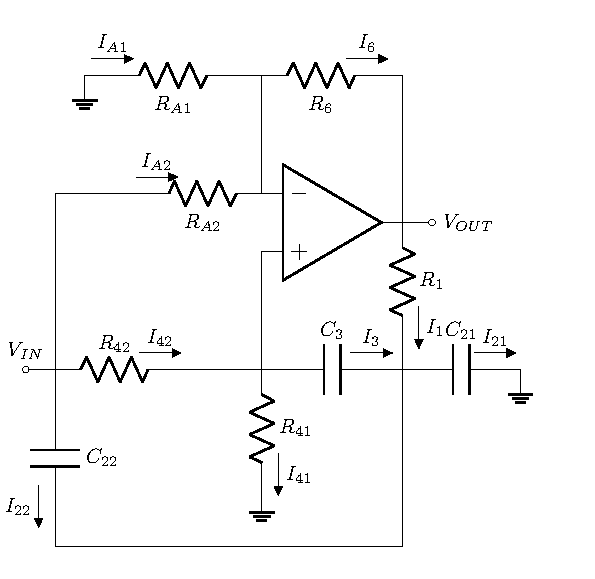
\includegraphics[width=0.5\textwidth]{Imagenes-Ej3/CircuitoDeGuido.pdf}
	\caption{Circuito celda.}
	\label{fig:HPBSedrac}
\end{figure}
Plantenado los siguientes nodos es posible llegar a la expresión de la función transferencia:
\begin{align}
\frac{-V^-}{R_{a1}}+\frac{V_{in}-V^-}{R_{a2}}=\frac{V^--V_{out}}{R_b}
\end{align}
\begin{align}
V^+=V^-
\end{align}
\begin{align}
\frac{V_{in}-V^+}{R_{42}}=\frac{V^+}{R_{41}}+sC_3\cdot (V^+-V_a)
\end{align}
\begin{align}
(V^+-V_a)\cdot sC_3 + (V_{in}-V_a)\cdot sC_{22}+\frac{V_{out}-V_a}{R_1}=V_a\cdot sC_{21}
\end{align}
\begin{align}
H(s)=
{\frac { \alpha +s \beta +{s}^{2} \gamma }{\delta+s \epsilon +{s}^{2} \zeta }
}
\end{align}


\begin{align}
\alpha = {\it R_{a2}}\,{\it R_B}\,{\it R_{41}}-{\it R_{a1}}\,{\it R_b}\,{\it R_{42}}+{
\it R_{a1}}\,{\it R_{a2}}\,{\it R_{42}}
\end{align}
\begin{align}
\beta =\left( {\it C_3}\,{\it R_{a1}}\,{\it R_{a2}}\,{
\it R_{41}}\,{\it R_1}-{\it C_3}\,{\it R_{a1}}\,{\it R_b}\,{\it R{_41}}\,{\it R_{42}}-{
\it C_3}\,{\it R_{a1}}\,{\it R_b}\,{\it R_{42}}\,{\it R_1}+{\it C_3}\,{\it R_{a2}}\,{
\it R_b}\,{\it R_{41}}\,{\it R_1} \right)
\end{align}
\begin{align}
\gamma = \left( -{\it C_{21}}\,{\it C_3
}\,{\it R_{a1}}\,{\it R_b}\,{\it R_{41}}\,{\it R_{42}}\,{\it R_1}+{\it C_{22}}\,{\it C_3}
\,{\it R_{a1}}\,{\it R_{a2}}\,{\it R_{41}}\,{\it R_{42}}\,{\it R_1}+{\it C_{22}}\,{\it C_3}
\,{\it R_{a2}}\,{\it R_b}\,{\it R_{41}}\,{\it R_{42}}\,{\it R_1} \right) 
\end{align}
\begin{align}
\delta = {\it R_{a1}}
\,{\it R_{a2}}\,{\it R_{42}}+{\it R_{a1}}\,{\it R_{a2}}\,{\it R_{41}} 
\end{align}
\begin{align}
\epsilon = \eta +  \iota
\end{align}
\begin{align}
\eta ={\it C_3}\,{\it R_{a1}}\,{\it R_{a2}}\,{\it R_{41}}\,{\it R_{1}}+{\it C_3}\,{\it R_{a1}}\,{\it R_{a2}}\,{\it R_{42}}\,{\it R_1}-{\it C_3}\,{\it R_{a1}}\,{\it R_b}\,{\it R_{41}}\,{\it R_{42}}-{
\it C_3}\,{\it R_{a2}}\,{\it R_b}\,{\it R_{41}}\,{\it R_{42}}
\end{align}
\begin{align}
\iota={\it C_{21}}\,{\it R_{a1}}\,{
\it R_{a2}}\,{\it R_{41}}\,{\it R_1}+{\it C_{21}}\,{\it R_{a1}}\,{\it R_{a2}}\,{\it R_{42}}\,{
\it R_1}+{\it C_{22}}\,{\it R_{a1}}\,{\it R_{a2}}\,{\it R_{41}}\,{\it R_1}+{\it C_{22}}\,{
\it R_{a1}}\,{\it R_{a2}}\,{\it R_{42}}\,{\it R_1}
\end{align}
\begin{align}
\zeta = \left( {\it C_{21}}
\,{\it C_3}\,{\it R_{a1}}\,{\it R_{a2}}\,{\it R_{41}}\,{\it R_{42}}\,{\it R_1}+{\it C_{22}}
\,{\it C_3}\,{\it R_{a1}}\,{\it R_{a2}}\,{\it R_{41}}\,{\it R_{42}}\,{\it R_1} \right)
\end{align}
\subsubsection{Elecciones de diseño}
Cada una de las funciones transferencia descriptas en (\ref{eq:trans}) pueden ser expresadas de la siguiente manera:
\begin{align}
	H_i(s)=\frac{G_\infty (s^2+\omega_z^2)}{s^2+\frac{\omega_0 \cdot s}{Q}+\omega_0^2}
\end{align} 

Luego, siguiendo con el análisis matemático desarrollado en el paper ``Optimum Configurations for Single Amplifiers Biquadratic Filters'', se ve la necesidad de introducir algunos parámetros, los cuales permiten el diseño de la celda. Estos son $G_\infty$, el cual es la ganancia cuando $\omega \rightarrow \infty$, K y $Q_0$, siendo esta ultima una constante que debe cumplir la condición $Q_0 < Q$. Es así que permite ajustar el valor de los componentes. Se eligió el valor de $Q_0$ en base a una relación de dependencia con las sensibilidades. Luego se definen los parámetros de interés, presentados a continuación. 
\begin{equation}
	k=\frac{G_\infty\cdot \left(\frac{\omega_z}{\omega_0} \right)^2}{1-\frac{Q_0}{Q}}
\end{equation}
\begin{equation}
	K=1+\frac{1-\frac{Q_0}{Q}}{2\cdot Q_0^2}
\end{equation}
\begin{equation}
	n= k\cdot (1-\frac{Q_0 }{K\cdot Q})
\end{equation}
\begin{equation}
	m=  \left( k-\frac{k}{K} \right) \cdot \left[1+2\cdot \left(\frac{Q_0\cdot \omega_0}{\omega_z}\right)^2 \right]
\end{equation}

A partir de aquí, y asignando valores para $Q_0$, C y $R_b$, se puede obtener los valores para el resto de las variables con dichas equivalencias.  
\begin{equation}
	R_a= \frac{1}{(K-1) R_b}
\end{equation}
\begin{equation}
	R_{a1}=\frac{1}{(1-k)\cdot R_a}
\end{equation}
\begin{equation}
	R_{a2}=\frac{1}{k \cdot R_a}
\end{equation}
\begin{equation}
	R_{41}=	\frac{1}{(1-n)\cdot R_4}
\end{equation}
\begin{equation}
	R_{42}=	\frac{1}{n\cdot R_4}
\end{equation}
\begin{equation}
	C_{21} = (1-m) \cdot C
\end{equation}
\begin{equation}
	C_{22} = m \cdot C
\end{equation}

Se presenta a continuación el análisis de sensibilidades del circuito, el cual coincide con lo publicado en el paper: 
\begin{table}[H]
\centering
\begin{tabular}{ccc}
\hline
Componente & $S^\omega_0$ & $S^Q$                                      \\ \hline
$S_{R_1}$  & -0.5         & $-\left( \frac{Q}{Q_0} -0.5 \right)$       \\
$S_{C}$    & -0.5         & $0.5\cdot \left( \frac{Q}{Q_0} -1 \right)$ \\
$S_{R_4}$  & -0.5         & $\left( \frac{Q}{Q_0} -0.5 \right)$        \\
$S_{R_a}$  & 0            & $-\left( \frac{Q}{Q_0} -1 \right)$         \\
$S_{R_b}$  & 0            & $\left( \frac{Q}{Q_0} -1 \right)$         \\
\hline
\end{tabular}
\caption{Cuadro de sensibilidades del filtro.}
\label{tab:sensibilidad}
\end{table}

En base a lo expuesto en la Tabla (\ref{tab:sensibilidad}), se tomó especial cuidado en la elección de componentes y en el matcheo de impedancias. De esta forma, se tomaron como valor de los componentes los presentados a continuación:
\begin{table}[H]
\centering
\begin{tabular}{ccccc}
\hline
\multicolumn{1}{c}{Componente} & \multicolumn{1}{c}{1er Etapa} & \multicolumn{1}{c}{Composición} & 2da Etapa        & Composición            \\ \hline
$R_{a1}$                          & 12.36 k$\Omega$               & 330 + 12 k$\Omega$                & 6.2 k$\Omega$    & (1.5 + 4.7) k$\Omega$   \\
$R_{a2}$                          & 100 k$\Omega$                 & 100 k$\Omega$                   & 89.67 k$\Omega$ & (22 + 68) k$\Omega$     \\
$R_b$                          & 50.72 k$\Omega$              & (3.9 + 47) k$\Omega$             & 1 k$\Omega$       & 1 k$\Omega$             \\
$R_{41}$                          & 23.88 k$\Omega$               & (1.8 + 22) k$\Omega$               & 203.36 k$\Omega$ & (270 // 820) k$\Omega$ \\
$R_{42}$                          & 207 k$\Omega$                 & (27 + 180) k$\Omega$             & 4.19 M$\Omega$   & (1.8 + 2.2) M$\Omega$   \\
$R_1$                          & 74.05 k$\Omega$               & (18 + 56) k$\Omega$              & 25.07 k$\Omega$  & (10 + 15) k$\Omega$       \\
$C_3$                          & 100 pF                        & 100 pF                          & 100 pF           & 100 pF                 \\
$C_{21}$                          & 74.14 pF                      & (18 // 56) pF                    & 18.52 pF         & (22 + 120) pF           \\
$C_{22}$                          & 25.86 pF                       & (33 + 120) pF                    & 81.48 pF          & (82p +12n) F         \\
\hline    
\end{tabular}
\caption{Componentes seleccionados.}
\label{tab:componentes}
\end{table}

Además, se calculó el error porcentual asociado a la aproximación de las impedancias.
\begin{table}[H]
\centering
\begin{tabular}{ccc}
\hline
\multicolumn{1}{c}{Error Porcentual} & \multicolumn{1}{c}{1er Etapa} & \multicolumn{1}{c}{2da Etapa} \\ \hline
$R_{a1}$                                & 0.2 $\%$                      & $\approx 0 \%$                \\
$R_{a2}$                                & $\approx 0 \%$                & 0.4 $\%$                      \\
$R_b$                                & 0.4 $\%$                      & $\approx 0 \%$                \\
$R_{41}$                                & 0.3 $\%$                      & 0.1 $\%$                      \\
$R_{42}$                                & $\approx 0 \%$                & 0.3 $\%$                      \\
$R_1$                                & 0.1 $\%$                      & 0.3 $\%$                      \\
$C_3$                                & $\approx 0 \%$                & $\approx 0 \%$                \\
$C_{21}$                                & 0.2 $\%$                      & 0.4 $\%$                      \\
$C_{22}$                                & 0.1 $\%$                      & 0.1 $\%$        \\
\hline
\end{tabular}
\caption{Error porcentual de los componentes.}
\end{table}

Un criterio utilizado para seleccionar dichos valores fue tomar capacitores pequeños, dado a que ellos son mas certeros y no varían tanto frente a la temperatura. En base a esto, definir el resto de los componentes.  

\subsubsection{Acoplamiento de Impedancias}
Para que ambas etapas no se carguen entre si, la impedancia de entrada de la segunda etapa debe ser mucho mayor a la de salida de la primera. De esta forma, se simuló la impedancia de entrada de ambas etapas.
\begin{figure}[H]
	\centering
	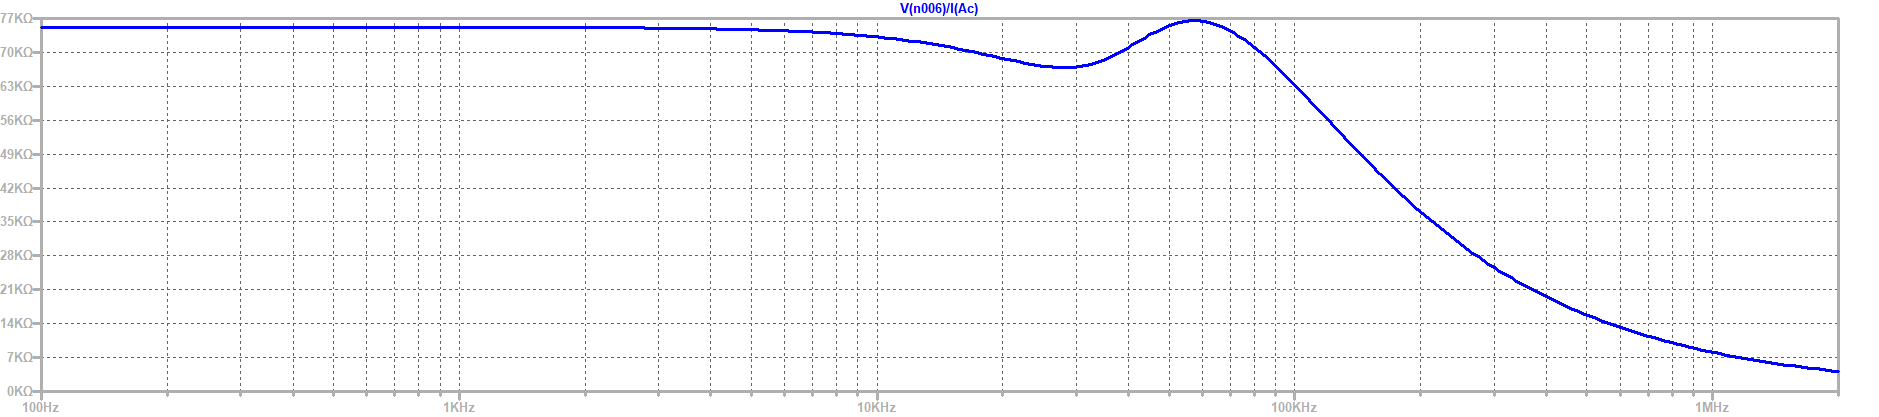
\includegraphics[width=\textwidth]{Imagenes-Ej3/ZinE1.png}
	\label{fig:zine1}
	\caption{Impedancia de entrada de la primer etapa.}
\end{figure}
\begin{figure}[H]
	\centering
	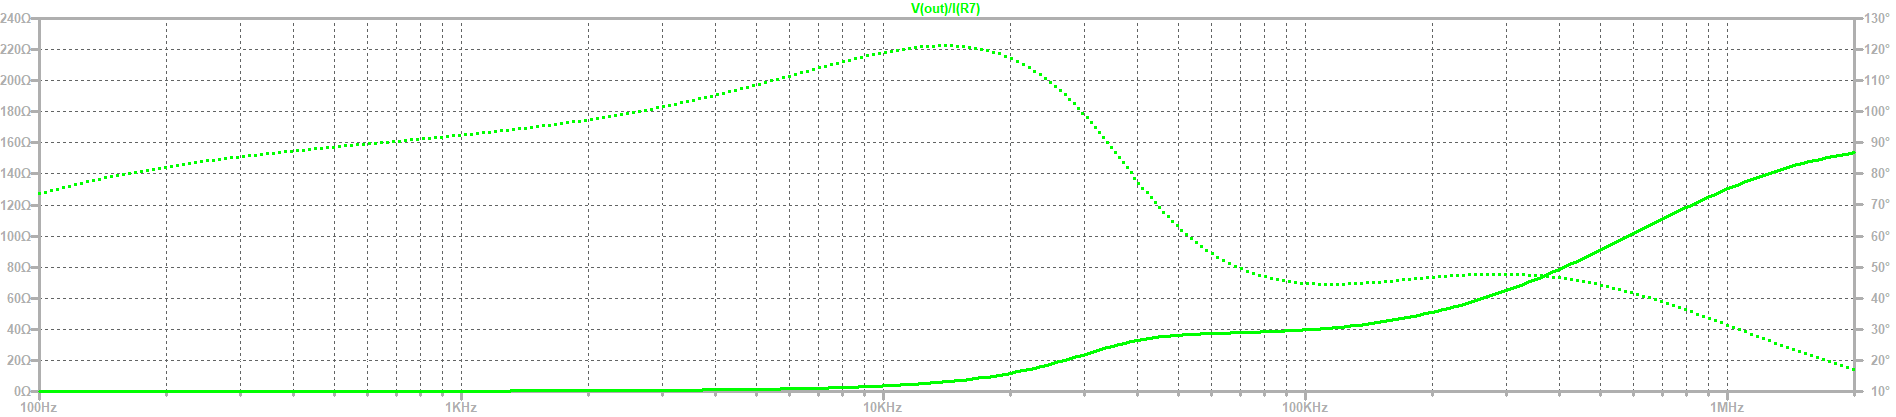
\includegraphics[width=\textwidth]{Imagenes-Ej3/ZoutE1.png}
	\label{fig:zoute1}
	\caption{Impedancia de salida de la primer etapa.}
\end{figure}
\begin{figure}[H]
	\centering
	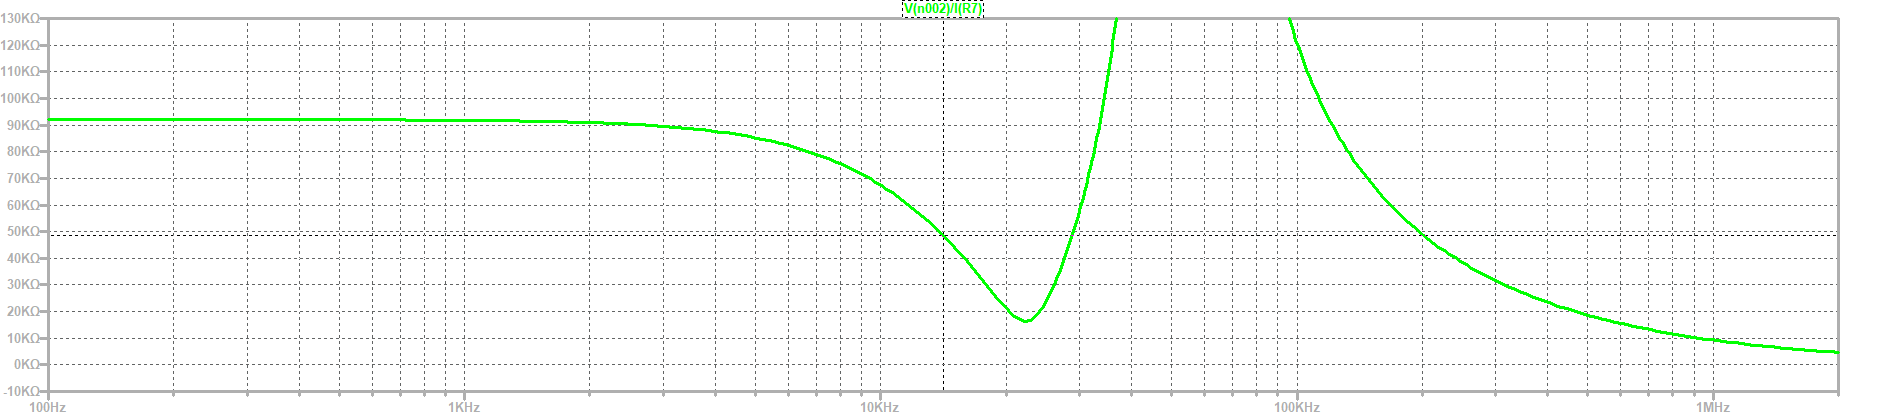
\includegraphics[width=\textwidth]{Imagenes-Ej3/ZinE2.png}
	\label{fig:zine2}
	\caption{Impedancia de entrada de la segunda etapa.}
\end{figure}

Se puede concluir, luego de estas gráficas, que el acoplamiento de impedancias de da adecuadamente, por lo tanto se decidió no utilizar un buffer para conectar cada etapa.

\subsection{Respuesta en Frecuencia}
Se realizó un análisis de Montecarlo a la respuesta en frecuencia del circuito, utilizando una tolerancia de las resistencias al $1\%$ y capacitores al $10\%$, obteniendo la siguiente dispersión.
\begin{figure}[H]
	\centering
	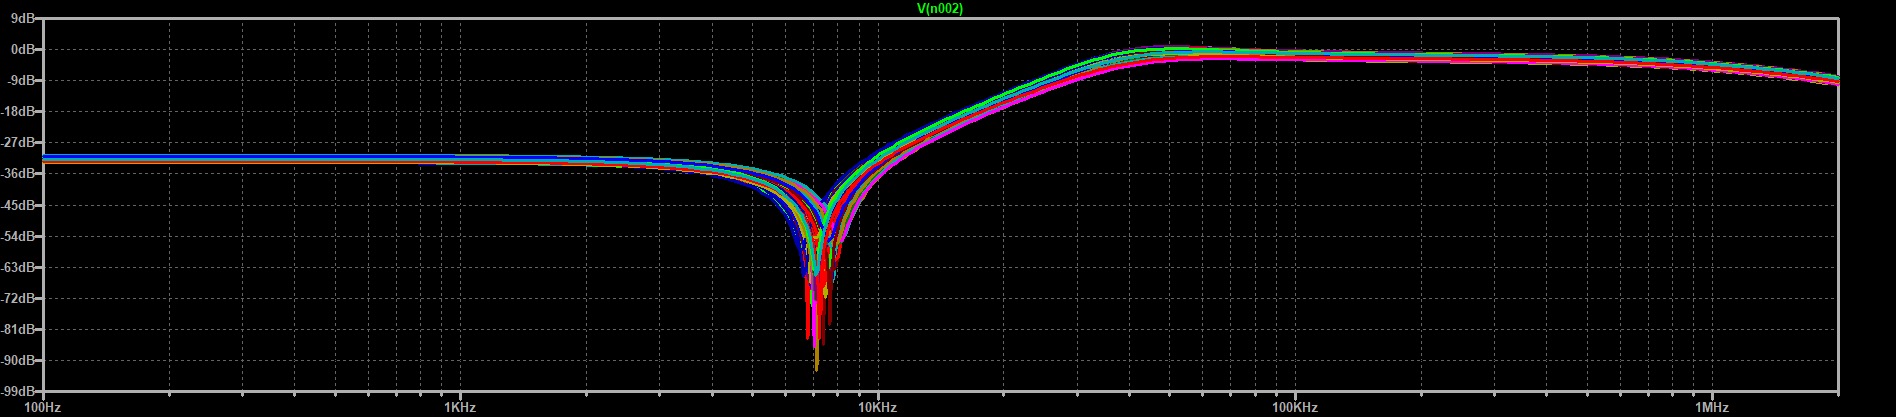
\includegraphics[width=\textwidth]{Imagenes-Ej3/mcsedra.png}
	\label{fig:mcsedra}
	\caption{Análisis de Montecarlo Filtro entero.}
\end{figure}
Se puede apreciar una dispersión en la frecuencia de corte del sistema. Es a causa de esto que se tuvo en cuenta en el diseño el hecho de utilizar un preset, con el propósito de poder ajustar el filtro. Un problema que se presenta con esta metodología es que, no solamente importa la ubicación del cero de transmisión, sino que también el $Q$ presente. Para poder solucionar esta problemática, se utiliza un preset en cada etapa. En la primera, el componente es colocado sobre $R_1$, dado a que la sensibilidad de $\omega_z$ depende de esta. Por otro lado, en la segunda etapa, es decir, la de mayor Q, se lo coloca en la resistencia $R_b$. Dado que se decidió medir el circuito previamente a la colocación de los presets, es decir, con resistencias fijas, y dado a que el mismo cumplía con las especificaciones, se tomo la decisión de no utilizar los componentes variables.
 
\subsubsection{Etapas}
Además del Montecarlo del filtro en su totalidad, se realizó el mismo análisis para cada etapa por separado.
\begin{figure}[H]
	\centering
	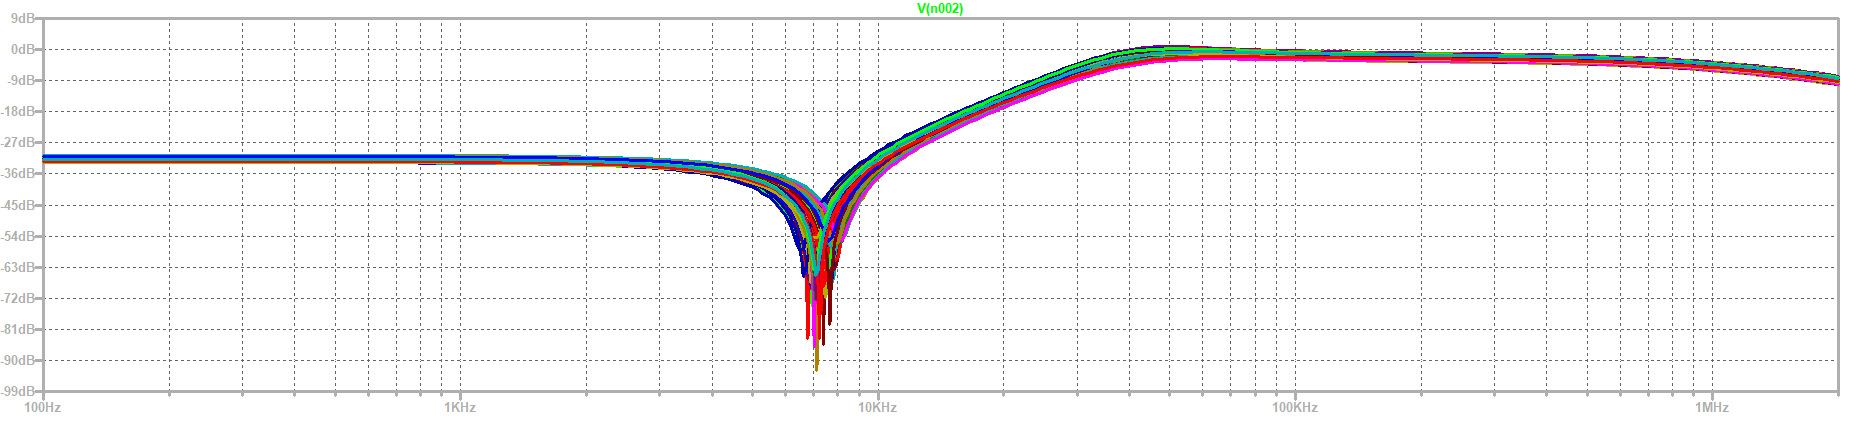
\includegraphics[width=\textwidth]{Imagenes-Ej3/mcsedraE1.png}
	\caption{Análisis de Montecarlo de la primer etapa.}
	\label{fig:mcsedrae1}
\end{figure}
En la Figura (\ref{fig:mcsedrae1}) se puede observar como la dispersión modifica seriamente el Q tanto como la posición del cero de transmisión.
\begin{figure}[H]
	\centering
	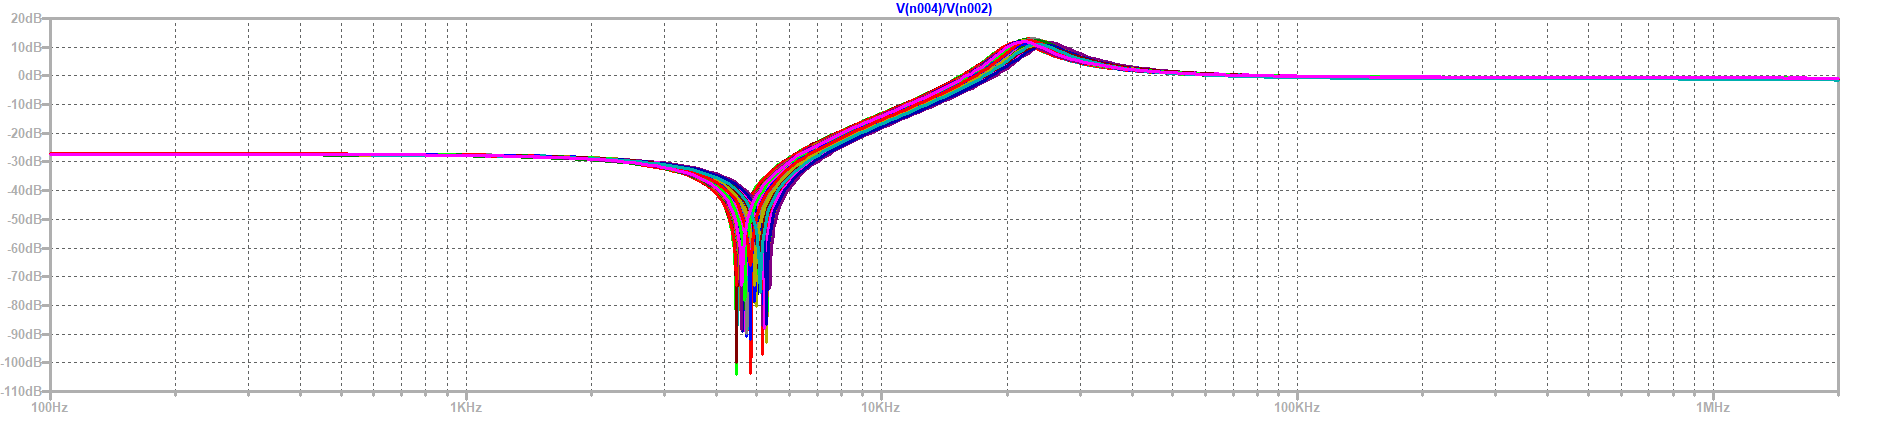
\includegraphics[width=\textwidth]{Imagenes-Ej3/mcsedraE2.png}
	\caption{Análisis de Montecarlo de la segunda etapa.}
	\label{fig:mcsedrae2}
\end{figure}
Por otro lado, se puede apreciar en la Figura (\ref{fig:mcsedrae2}) que la altura del sobrepico posee una gran dispersión, si bien los valores de la transferencia para $s\rightarrow 0$ y $s\rightarrow \infty$ son aproximadamente constantes mas allá de la dispersión.

Luego, se hicieron simulaciones de como el preset podría ser utilizado para variar el Q del circuito, comenzando por utilizar un preset en la primer etapa sobre $R_1$, como se mencionó previamente.
\begin{figure}[H]
	\centering
	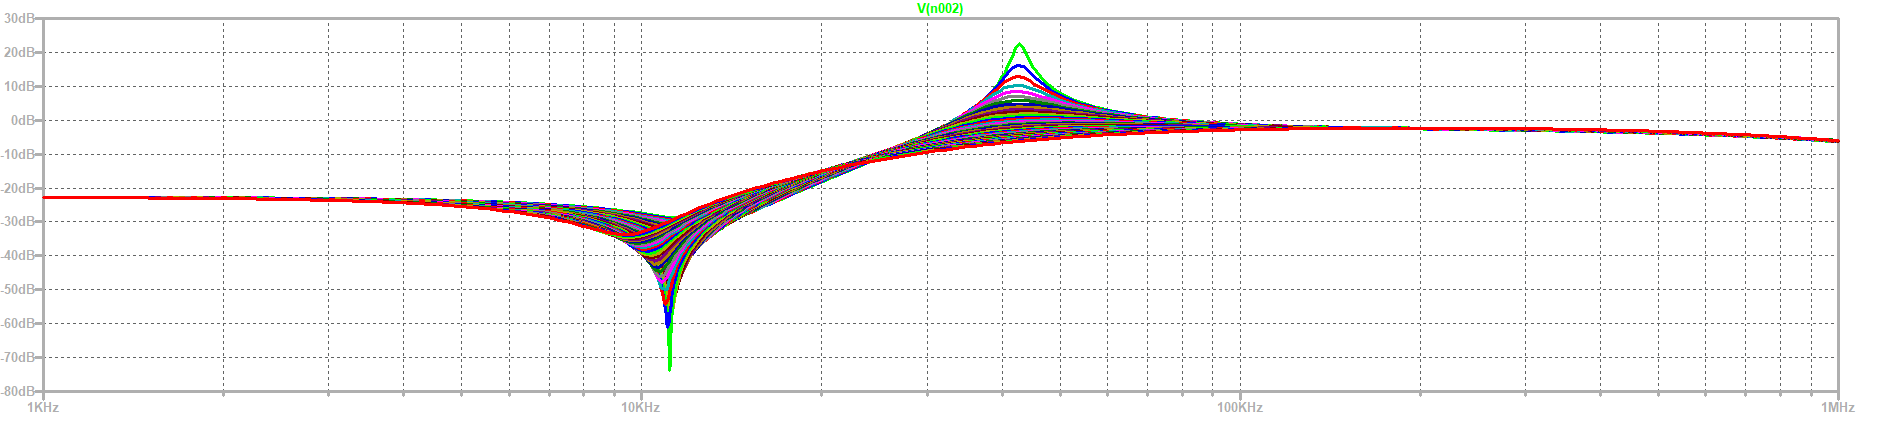
\includegraphics[width=\textwidth]{Imagenes-Ej3/mcPoteR6E1.png}
	\label{fig:presete1}
	\caption{Análisis uso de preset primer etapa.}
\end{figure}
De aquí se puede concluir que la utilización de un preset en esta etapa ayuda a fijar tanto a un Q como a ajustar el cero de transmisión.

Luego se prosiguió con la segunda etapa, sobre la resistencia $R_b$:
\begin{figure}[H]
	\centering
	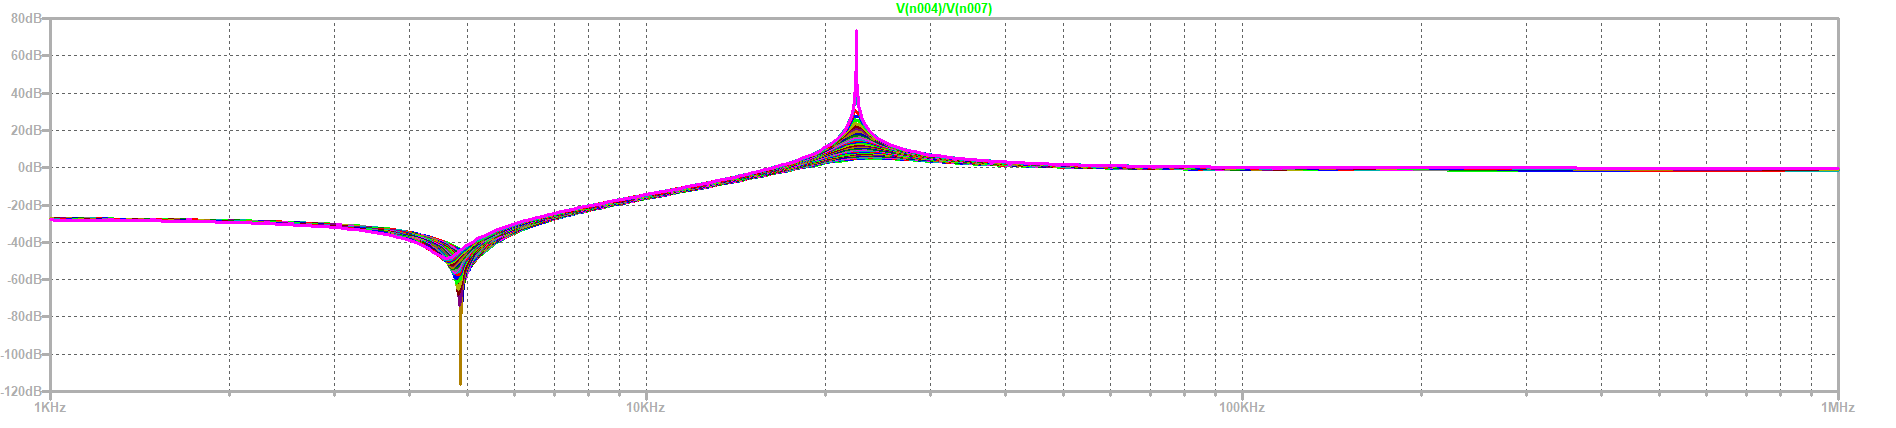
\includegraphics[width=\textwidth]{Imagenes-Ej3/mcPoteR3E2.png}
	\label{fig:presete2}
	\caption{Análisis uso de preset segunda etapa.}
\end{figure}

De aquí, como era esperado, se ve que esta etapa tiene una mayor sensibilidad respecto a Q, lo cual implica que idealmente se debe utilizar un preset para ajustarlo.

Además, dado a que inicialmente se realizó el filtro y cumplía las especificaciones, se decidió no utilizar un preset, como ya se había mencionado. Sin embargo, se tuvo la precaución de diseñar una etapa de compensación de ganancia para el caso en el que la variación de las condiciones ambientales modifique el filtro, resultando esta necesaria. Dicha etapa consiste en un no inversor con ganancia variable.

Luego se realizó un histograma para la frecuencia de los polos, datos extraídos del análisis de Montecarlo, donde el eje Y es el porcentaje de la probabilidad de aparición y el X es la frecuencia.
\begin{figure}[H]
	\centering
	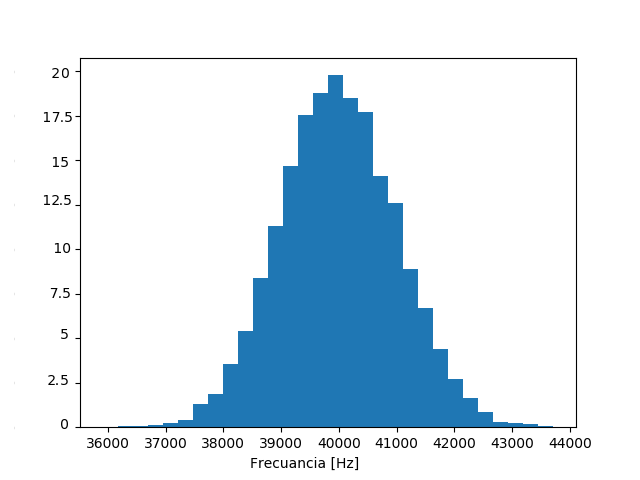
\includegraphics[width=0.5\textwidth]{Imagenes-Ej3/histW01.png}
	\caption{Histograma primer polo.}
	\label{fig:hist1}
\end{figure}
\begin{figure}[H]
	\centering
	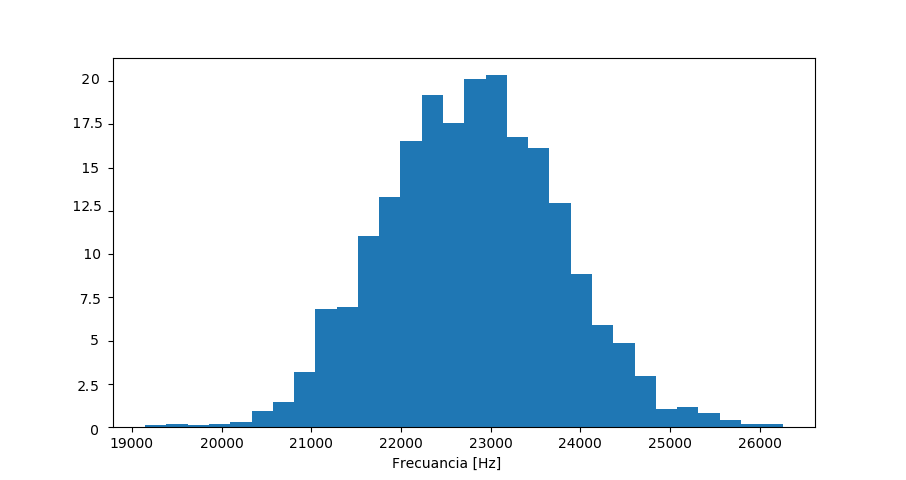
\includegraphics[width=0.7\textwidth]{Imagenes-Ej3/histW02.png}
	\caption{Histograma segundo polo.}
	\label{fig:hist2}
\end{figure}

\subsubsection{Filtro definitivo}
Se realizó el filtro obteniendo la siguiente respuesta en frecuencia 
\begin{figure}[H]
	\centering
	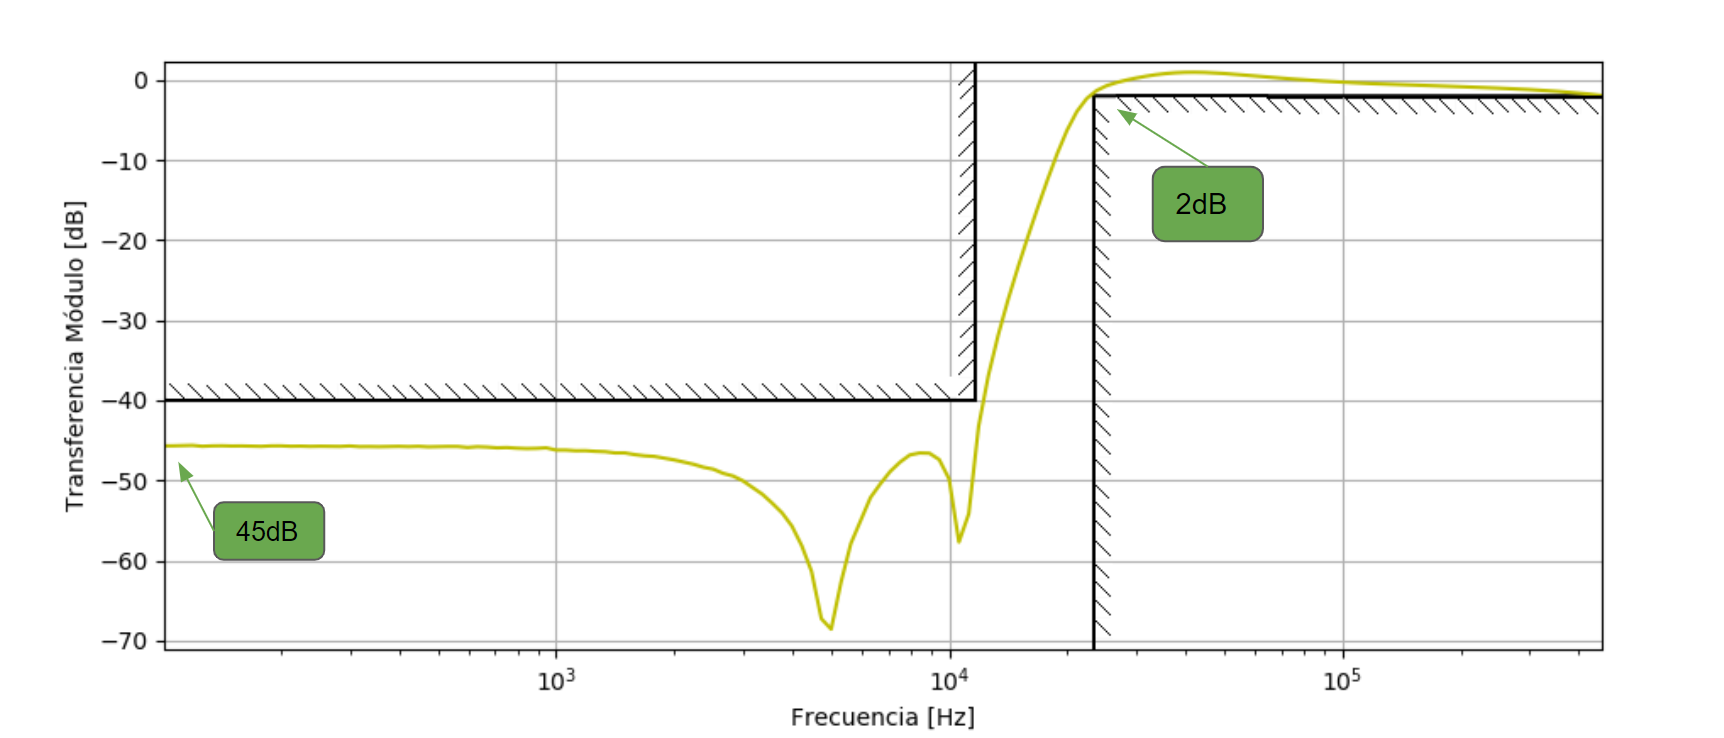
\includegraphics[width=\textwidth]{Imagenes-Ej3/BodeSedra.png}
	\caption{Filtro High-Pass en módulo.}
	\label{fig:BodeSedra}
\end{figure}
\begin{figure}[H]
	\centering
	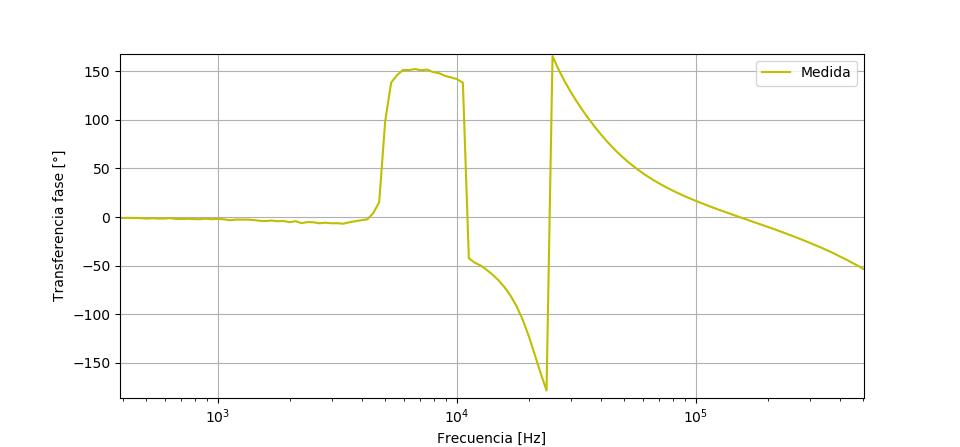
\includegraphics[width=\textwidth]{Imagenes-Ej3/FaseBodeSedra.png}
	\label{fig:FaseBodeSedra}
	\caption{Filtro High-Pass en fase}
\end{figure}

Se destaca de la Figura (\ref{fig:BodeSedra}) que el filtro realizado efectivamente cumple la plantilla deseada. También puede tomarse en cuenta que los resultados obtenidos se corresponden con lo simulado y calculado de forma teórica:
\begin{figure}[H]
	\centering
	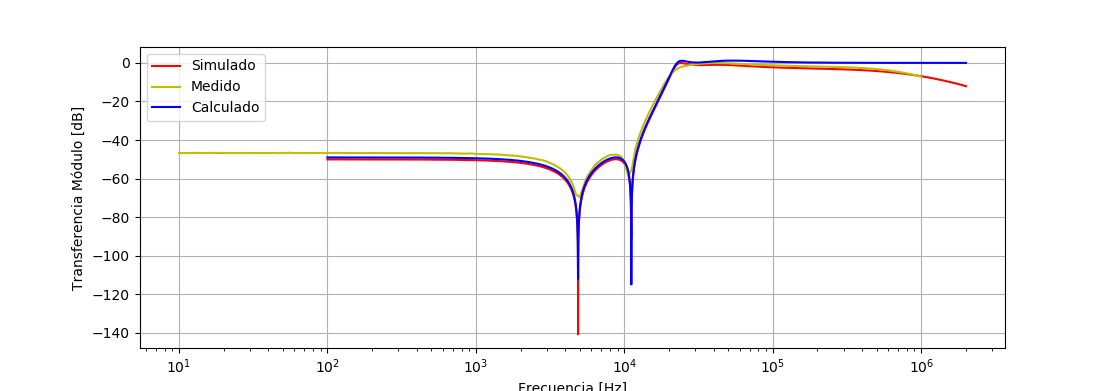
\includegraphics[width=\textwidth]{Imagenes-Ej3/BodeMedCalcSim.png}
	\caption{Comparación del filtro High-Pass en módulo.}
	\label{fig:BodeSedraComp}
\end{figure}
\begin{figure}[H]
	\centering
	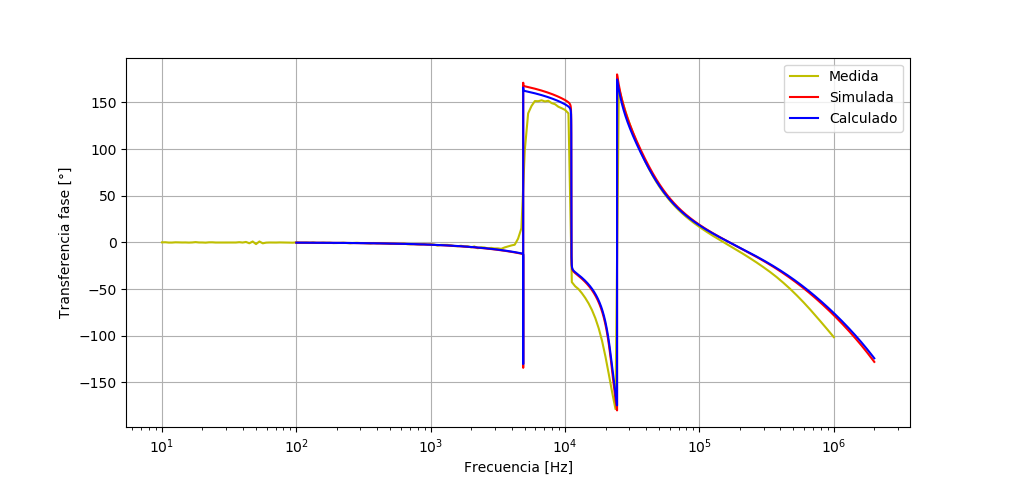
\includegraphics[width=\textwidth]{Imagenes-Ej3/BodeMedCalcSimFase.png}
	\label{fig:FaseBodeSedraComp}	
	\caption{Comparación del filtro High-Pass en fase.}
\end{figure}

\subsection{Rango Dinámico}
El rango dinámico se define como la razón de máximo y mínimo valor que puede tomar un observable de interés. Para el caso en cuestión, queda definido de la siguiente manera:
\begin{align}
	R_d = 20 \log_{10} \left( \frac{V_{in_{max}}}{V_{in_{min}}} \right)
\end{align}

Para definir $V_{in_{min}}$, se tuvo en cuenta la tensión mínima que se pudo distinguir respecto al piso de ruido, la cual es de $V_{in_{min}} \approx 10 \ mV$. Luego, para el caso de $V_{in_{max}}$, se tuvo en cuenta la máxima tensión previa a la aparición de alinealidades, siendo estos efectos el cross-over, slew-rate y saturación del amplificador operacional. Dos de estos problemas son solucionados mediante la elección del integrado, ya que se utiliza un TL081, el cual tiene un slew-rate elevado y no posee el problema del cross-over debido a su etapa de salida. Por su parte, para el problema de la saturación, es de utilidad saber que la máxima tensión de salida es $V_{sat} = Vcc - 1.5 \ V = 13.5 \ V$. Para encontrar el valor de tensión máximo de entrada se consideró la ganancia del sistema y, teniendo en cuenta la conexión entre etapas, este factor queda definido por la siguiente expresión:
\begin{align}
V_{in_{max}}=\frac{V_{sat}}{  \max(G_{E1} \cdot G_{E2} )} = 13V
\end{align}
Es así que con lo mencionado previamente, se obtiene $R_d = 62.2dB$.

\subsection{Estabilidad}
Se buscó en esta sección lograr que la celda oscile, introduciéndole una señal cuadrada, la cual es sabido que está compuesta por un gran numero de frecuencias. De esta forma, y variando, no solo la amplitud de la misma sino también su frecuencia y duty-cycle, no se pudo hacer oscilar a la celda. La siguiente imagen es la respuesta de la celda al escalón.
\begin{figure}[H]
	\centering
	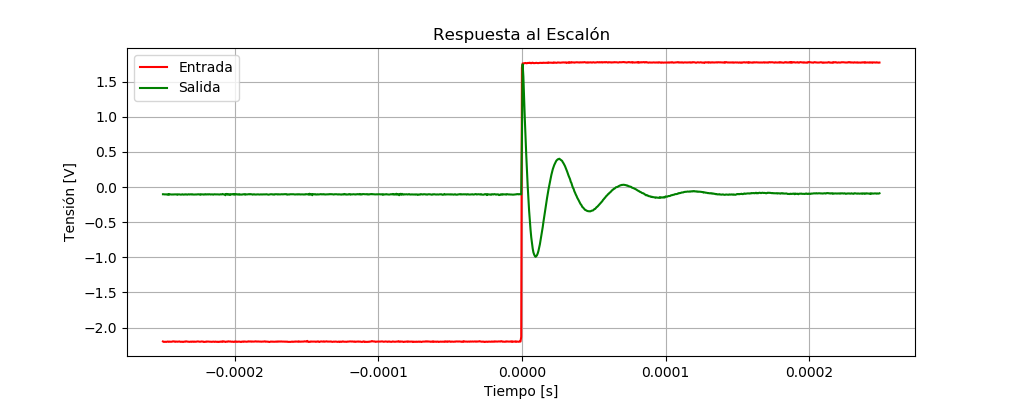
\includegraphics[width=\textwidth]{Imagenes-Ej3/Step.png}
	\label{fig:stepresponse}
	\caption{Respuesta al escalón del circuito.}
\end{figure}

\subsection{Conclusiones}
La celda Sedra es una gran alternativa cuando no se tiene un amplificador operacional con una ganancia a lazo abierto relativamente estable. También permite la implementación de un filtro de segundo orden con tan solo 1 operacional, mientras que por ejemplo la celda universal utiliza 3 de ellos en el mejor de los casos. Además, cuenta con el beneficio de poder sintetizar valores de Q relativamente altos gracias a su doble realimentación, tanto negativa como positiva, dando esta última una de sus desventajas, la cual consiste en la posibilidad de que haya una oscilación en el circuito.